\section{Introduction}
Inverse photoemission spectroscopy (IPES) is a powerful technique for condensed matter physics. It is the conjugate technique to angle resolved photoemission spectroscopy (ARPES)
and grants access to the unoccupied electronic states that ARPES does not access. As a brief overview, a sample in an ultra high vacuum environment is bombarded with
electrons of a known energy from an electron gun. These electron are in a low energy range, typically 0eV to 100eV, meaning that their penetration depth into the sample is very low; making
IPES a surface sensitive technique. If the electron energy matches an energy state available in the unoccupied states (above the Fermi level) of the sample, then the 
incoming electrons will fill in those states. These excited states then undergo a radiative relaxation which leads to the release of a UV photon. If a photon is radiated within the
solid angle of a detector's viewing angle then it will pass through the entrance window and lead to a detection. So IPES is a method of varying incident electron energy and recording
the subsequent count rate, with a high count rate at a given energy indicating the presence of an unoccupied state at that energy. There are three main components to obtaining good 
results from an IPES experiment: a good quality surface of the sample, a minimal thermal energy spread and size of the electron beam, and a small bandpass, with a high count rate and 
minimal breakdowns (arcing from anode to cathode) from the photodetectors. 

Inverse photoemission was first shown to be a viable experimental technique by John Pendry in 1981\cite{pendry1981theory}, with the main results from his paper showing that the yield of photons in an IPES
experiment is directly proportional to the yield of electrons in an ARPES experiment. The key difference being that the proportionality constant makes the photon yield much smaller 
than the electron yield and thus the count rates for an IPES experiment will be much smaller than the count rates for an ARPES experiment on the same sample. Taking this into consideration
with the three requirements listed above, it becomes apparent that a great deal of work needs to be put into optimizing the photodetection capabilities of the system. The overall goal
is to find a region in parameter space for each detector that yields a maximal count rate, subject to the constraint of minimizing detections caused from breakdowns within the detector. 
There are several parameters which can be varied about each detector, including the temperature of the entrance window, the dimensions of the tubes, distance to the sample, detection gas used, 
and the use of a quenching gas like Ar. However, for a GM tube operating at standard conditions we can greatly reduce the number of factors we need to consider varying. The tube 
design and counting gas have already been decided, and we have no way to vary the temperature of the entrance window; this leaves just the voltage applied to the anode of the detectors, 
and the pressure of the counting gas within the detectors. 

This report details our efforts to characterize how our photodetectors operate subject to different anode voltages and acetone pressures. We used LabVIEW to sweep through a set range of 
voltage values, and record the number of counts over a set amount of time. We did this with both the electron gun on and off; this allowed us to determine how many counts come from photons entering
the detector, and how many come from the tube arcing to itself. We then change the pressure of the acetone and repeat the process of scanning through the anode voltages. From this we can determine
the breakdown voltage of each tube at a given pressure, a quantity which denotes the anode potential at which the tube will begin to arc to itself. We can then examine the count rate of the tubes below 
this breakdown voltage to determine a stable region (minimal breakdowns) that maximize counts. 

\section{Background Theory}

\subsection{Inverse Photoemission (IPE)}
IPES and ARPES are both made possible by the photoelectric effect. First observed by Hertz and described by Einstein, the photoelectric effect is the emission of electrons from a sample
when light of sufficient energy is incident on it. The energy of the liberated electrons is given by $E_k = hf - \varphi$, where $hf$ is the incident photon energy, and $\varphi$ is the 
sample's work function. Inverse photoemission reverses this process, where electrons impinged on the sample are coupled to unoccupied electron states, and decay radiatively to yield a photon.
The energy of this photon is given by the change in the kinetic energy of the electron: $E_{ph} = hf = E_i - E_f$. 

If we consider the two processes together, we can see that one is simply the time reversal of the other. This is how Pendry\cite{pendry1981theory} went about showing the viability of IPES as an experimental technique. 
The scenario he used was as follows: find the probability that an electron with energy $E$, incident on a surface with angular coordinates $\theta$ and $\varphi$, emits a photon with 
energy $h\omega$ and polarization $s$. The intricacies of the calculations aren't important for understanding the results of this report, but his final result comparing photon and electron 
yields ($\mathscr{J}$) is as follows: 

\begin{equation}
\mathscr{J}_{el} = \frac{2Ec^2\cos\theta}{\omega^2\cos\Theta}\mathscr{J}_{ph}
\label{eq:pendry}
\end{equation}

The quantities $E$ and $\omega$ are fixed, leaving just the angles $\theta$ and $\Theta$, which are dependent solely on the geometry of the system. Ultimately this implies that photon yield from IPES experiments is small 
relative to the electron yield for an ARPES experiment. So to obtain the most accurate results we need to ensure that we `catch' as many photons in the detectors as possible, leading
to the photodetectors being one of the three main components for a successful IPE spectrometer. 

The use of low energy electrons for IPE must also be considered. \figref{IMFP} shows the calculated inelastic mean free path of an electron on Cu, Ag, and Au. This shows how far into
a sample an electron at a given energy would penetrate, giving the maximal depth of a sample that can be probed by IPES. 
\clearpage
\begin{figure}[h!]
\centering
\subcaptionbox{Electron IMFP against energy above Fermi level for Cu}[0.49\linewidth]{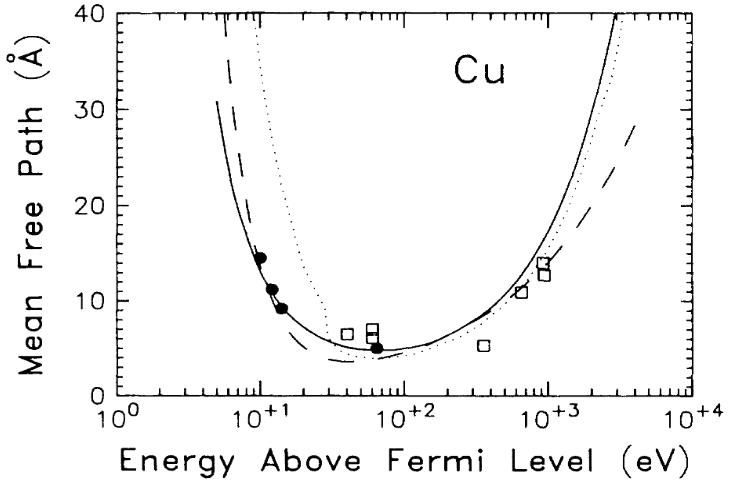
\includegraphics[scale=0.35]{Figs/IMFP Cu.png}}
\subcaptionbox{Electron IMFP against energy above Fermi level for Ag}[0.49\linewidth]{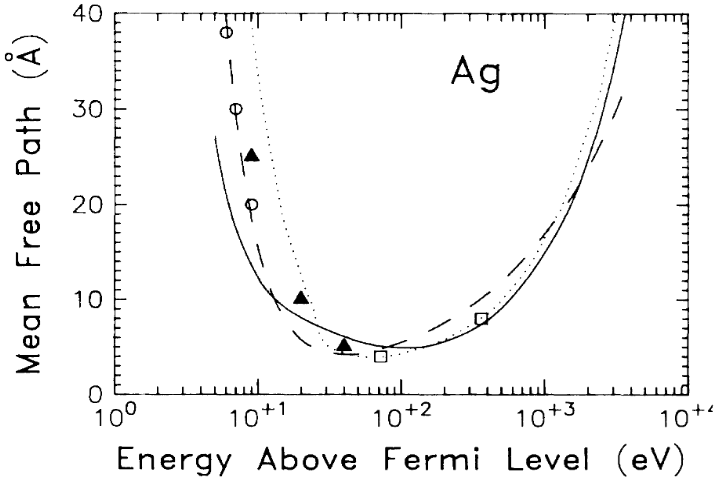
\includegraphics[scale=0.35]{Figs/IMFP Ag.png}}\\
\subcaptionbox{Electron IMFP against energy above Fermi level for Au}[0.49\linewidth]{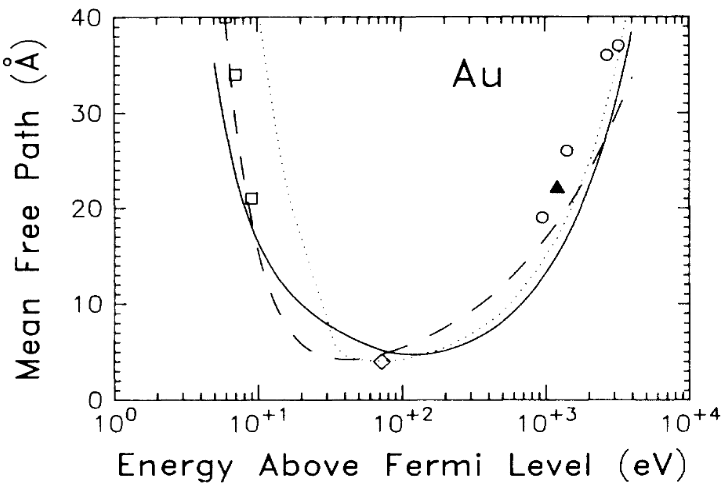
\includegraphics[scale=0.35]{Figs/IMFP Au.png}}
\caption{Mean free paths for electrons as a function of energy for various metals\cite{penn1987electron}}
\label{fig:IMFP}
\end{figure}

IPES uses electrons with an energy range typically between 10eV and 100eV which is the minimal mean free path for every sample present in the above plots. This means that the results
obtained during an IPES experiment are greatly influenced by the quality of the sample's surface. So a dirty sample, with solvent and gas molecules adsorbed to its surface 
could greatly reduce the amount of electrons which reach the surface of the sample. This is why the quality of the surface is another one of the three main components to good IPES 
results; meaning that we desire as clean and smooth a surface as possible. 

\subsection{Gas Filled Detectors}
There are two main ways of detecting the VUV photons released during inverse photoemission\cite{stiepel2005vacuum}: solid state detectors, and gas filled bandpass detectors. Most groups, including ours, opt
for the simpler and less expensive gas filled detectors. Most GM tubes for IPES follow a very similar design, with \figref{TubeDesign} showing the tube used by D Funnemann and H Merz
for their IPES setup. We will go over the design of the tubes briefly below, and will cover it more in depth during the experimental design section of this report. 

\begin{figure}[h!]
    \centering
    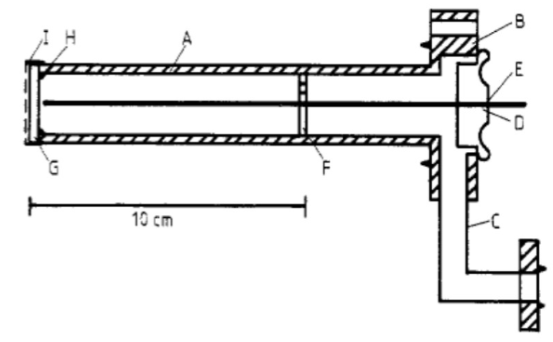
\includegraphics[scale=0.5]{Figs/tubedesign.png}
    \caption{Design diagram of GM tube\cite{funnemann198610}}
    \label{fig:TubeDesign}
\end{figure}

The design consists of a stainless steel tube which acts as the cathode of the detector and houses the internals of the detector. Within the tube is a tungsten wire which acts as the 
anode of the detector. Sealing the end of the tube is a window, made of either $\ce{MgF2}$ or $\ce{CaF2}$ which acts as the upper limit of the bandpass. The tube is pressurized with 
a counting gas; which in the case of our tubes is acetone. This acts as the lower end of the bandpass for the detector. To understand why this is the case, we need to cover the 
mechanism through which a GM tube operates. 

By biasing the anode wire, we create a cylindrical capacitor with an electric field going from the region of high potential (anode wire) to the region of low potential (the tube body).
The electric field can be found using Gauss' law, and is of the form:
\begin{equation}
\vec{E} = \frac{V}{r\ln\left(\frac{b}{a}\right)}\hat{r},
\label{eq:efield}
\end{equation}
where $r$ is the distance from the anode wire, $V$ is the potential applied to the anode, and $a$ and $b$ are the radii of the wire and tube respectively. The photons emitted from an IPES experiment are in the high
energy UV range (VUV), and are capable of ionizing the detection gas. This ionization leads to a positively charged gas ion, and a liberated electron. Based on the electric field 
in the detector, the ion is accelerated towards the tube wall while the electron is accelerated towards the anode wire. At the tube wall the gas ion picks up an electron and becomes 
a neutral gas molecule, ready to be used in a detection event again. If the potential of the anode is too low, the electron will simply be drawn towards it and one photon in will lead
to one electron reaching the detector. If the potential is large enough however, the accelerated electrons could ionize other gas molecules through collisions which leads to a multiplication
of the amount of electrons reaching the anode wire. This electron multiplication is known as a Townsend avalanche\cite{knoll2010radiation}, and is vital to producing a useable signal from the detector. It turns
what started of as a 1$e$ charge pulse, into one which could be on the order of tens of thousands of electron charge\cite{funnemann198610}.

The ionization potential of the counting gas determines the lower bound of the bandpass, since photons with a lower energy than this value are incapable of liberating the electrons 
which are detected at the output of the detector. The transmittance of the entrance window determines the upper bound of the bandpass, with the first instance of 0\% transmittance
indicating the cutoff of allowable photons. \figref{bandpass} shows the ionization potential of acetone, the transmittance of the entrance window, and their combined effect creating
the band of allowed energies for a GM tube.

\clearpage
\begin{figure}[h!]
    \centering
    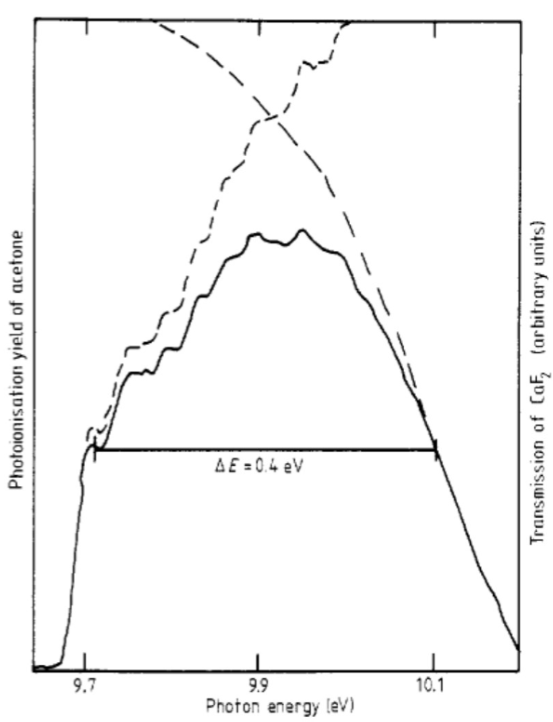
\includegraphics[scale=0.5]{Figs/bandpass.png}
    \caption{Energy band pass for an act. \ce{MgF2} GM tube, composed of contributions from the acetone ionization potential and transmittance of entrance window\cite{funnemann198610}}
    \label{fig:bandpass}
\end{figure}

GM tubes can operate in several different regimes based on the pressure of the detection gas and the applied voltage shown in \figref{gmmodes}.

\begin{figure}[h!]
    \centering
    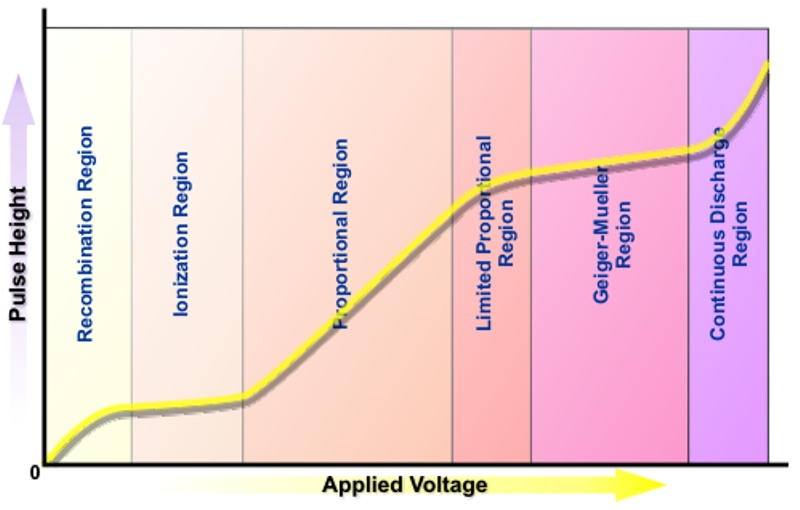
\includegraphics[scale=0.6]{Figs/gmmodes.jpg}
    \caption{Operating modes of GM tube over a range of anode voltages\cite{Conceptual}}
    \label{fig:gmmodes}
\end{figure}

For IPES, it is best to work in the proportional/limited proportional regime, though the Geiger region is also useable. The drawback of the Geiger region being that it is closer to the 
start of the continuous discharge region. Here the tube potential is so large that arcs can form between the anode and cathode without the need for photons to enter the tube. This
leads to spurious detections which could completely ruin the data collected in an IPES experiment. The onset of these discharges is the tube's breakdown voltage, and to obtain the 
cleanest (free from faulty detections) results we should only examine the tube's response to photons below this breakdown voltage. The operating mode of the GM tube can be determined
by analyzing the pulse height distribution of the detector. For a proportional tube we should expect to see the number of detections decrease as pulse height increases, and for a 
tube in the GM region we would expect a Gaussian type distribution about a mean pulse height value, since in the GM region we expect all pulses to have the same height due to complete
ionization of the gas surrounding the anode wire for every detection event. 
